\question \textbf{Select in $O(\log n)$}

Given the following Bitvector
\begin{align*}
    B = \left[11010110\,00001000\,00000010\,00000011\,00000000\,00001000\,00001011\,00010101\right]
\end{align*}

\begin{parts}
\part  Write down the blocks ($b = 8$) and superblocks ($s = 16$) for constant rank queries.

\begin{solution}

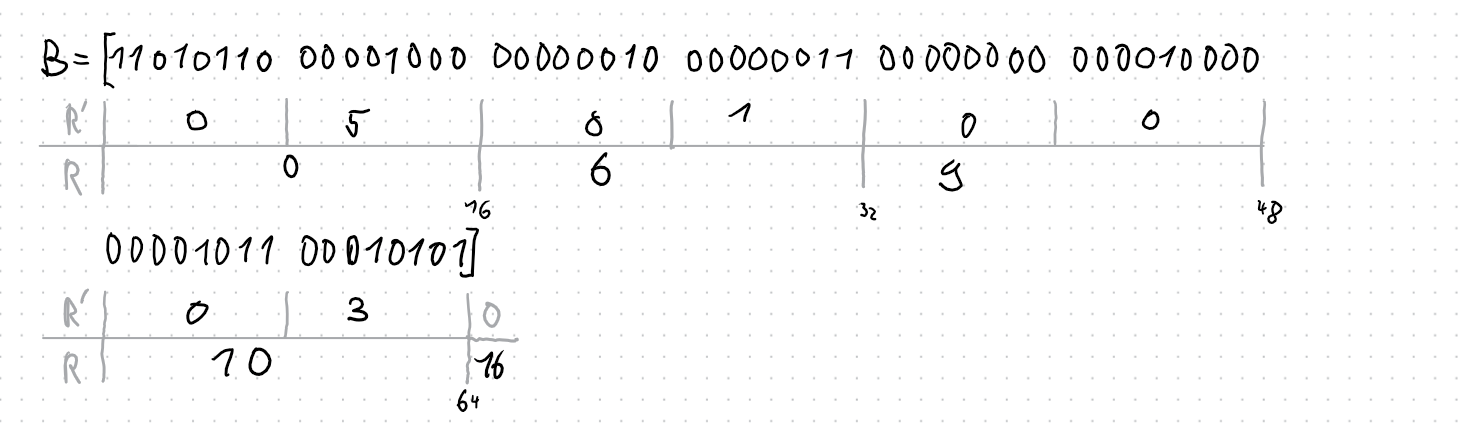
\includegraphics[width=\linewidth]{task_2/a6_a21.png}
\end{solution}

\part Write down the data structure $S$ to support select operations on the bitvector using 4 samples ($s = 4$).

\begin{solution}

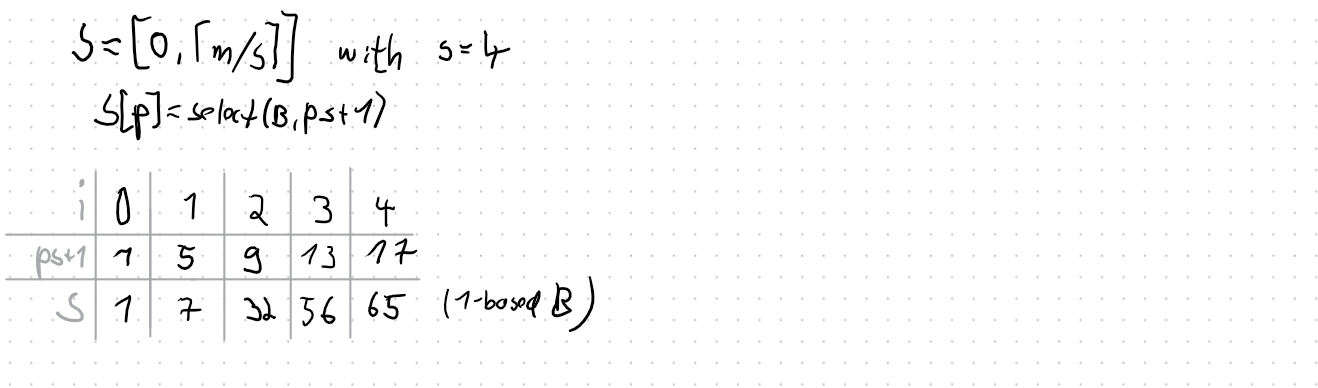
\includegraphics[width=\linewidth]{task_2/a6_a22.png}
\end{solution}

\part  Compute $\text{select}(B, 6)$ using your solution for S from above and conducting a binary search within a block (Note that the array $S$ is 0-based while $B$ is as always 1-based). Use rank queries when doing the binary search to query the amount of 1s up until your current position.

\begin{solution}

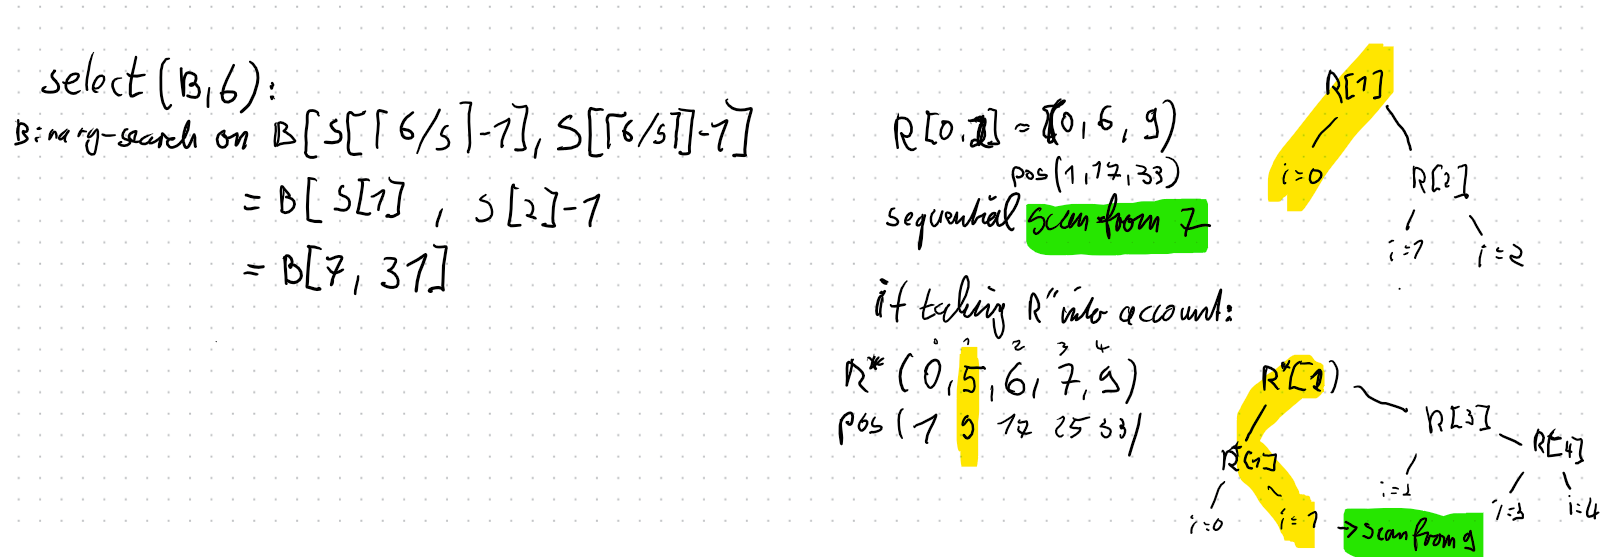
\includegraphics[width=\linewidth]{task_2/a6_a23.png}
\end{solution}
\end{parts}


% For tasks without simply remove the \begin{parts}...\part...\end{parts} commands